\section*{} %% bug workaround ...

\section{Il problema della rappresentazione grafica delle funzioni
complesse}\sectionmark{Rappresentaz. grafica di funzioni complesse} 

\`{E} tipico rappresentare le funzioni d'onda quantistiche mediante
il grafico del quadrato del modulo, sebbene in questo modo si perda
una parte dell'informazione. Il problema può essere risolto
cercando di superare le difficoltà tecniche relative
alla rappresentazione dei suoi valori complessi.

Un numero complesso può essere individuato dalla sua parte reale
e da quella immaginaria oppure dal modulo e dall'argomento. Sono comunque
necessarie due dimensioni spaziali per rappresentarlo graficamente. 
Sono possibili diverse soluzioni, a seconda della geometria e della
dimensionalità del sistema fisico.

Lo
stato dinamico di una particella quantistica in una dimensione
può essere descritto
da una funzione complessa definita sull'asse reale. Tale funzione 
può essere rappresentata mediante un grafico tridimensionale il
cui asse $x$ corrisponde alla variabile indipendente, mentre gli assi
$y$ e $z$ sono utilizzati per rappresentare le parti reale e immaginaria
del suo valore. 
%Alcuni esemp\^{i} sono illustrati in 
%\S \ref{sec:tunnel-graph}.
%
Alcuni esemp\^{i} verranno illustrati nel
prosieguo del capitolo (\S \ref{sec:tunnel-graph}).
%
%in Fig. \ref{fig:tunnel_first}-\ref{fig:tunnel_last}.
%
%, dove, per raffronto, 
%è riportata anche la usuale rappresentazione del modulo quadro (nel
%piano $xz$).

Per un sistema bidimensionale si avrebbe bisogno di quattro dimensioni:
in realtà è possibile realizzare il grafico tridimensionale di 
$|\Psi(x,y)|^2$ e servirsi di una scala di colori per rappresentare
l'argomento complesso. \`E necessario che gli estremi di questa scala
siano identificati --- corrispondano cioè allo stesso colore --- in modo
da evitare una errata percezione di discontinuità dell'argomento nel
passaggio da $-\frac{\pi}{2}$ a  $\frac{\pi}{2}$. Questa tecnica 
può essere utilizzata anche per rappresentare funzioni complesse di 
variabile complessa (funzioni analitiche, funzioni speciali etc.), di 
cui si fornisce un esempio in Fig. \ref{fig:zeta}. %Per quanto riguarda
%il sistema quantistico bidimensionale simulato nel presente lavoro, 
%alcuni fotogrammi significativi sono riportati nelle Figure 
%\ref{fig:comb1}-\ref{fig:comb4}.
\begin{figure}    
  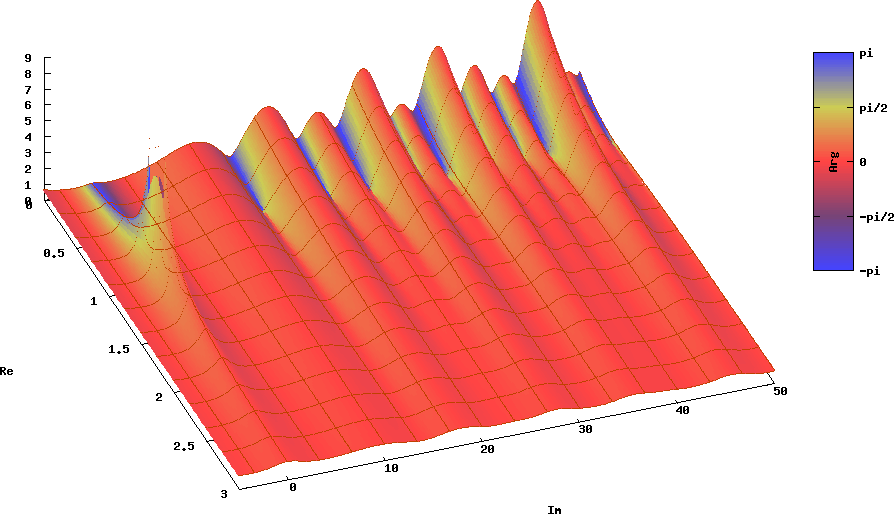
\includegraphics[width=60mm,height=30mm]{img/z/z0.png}
  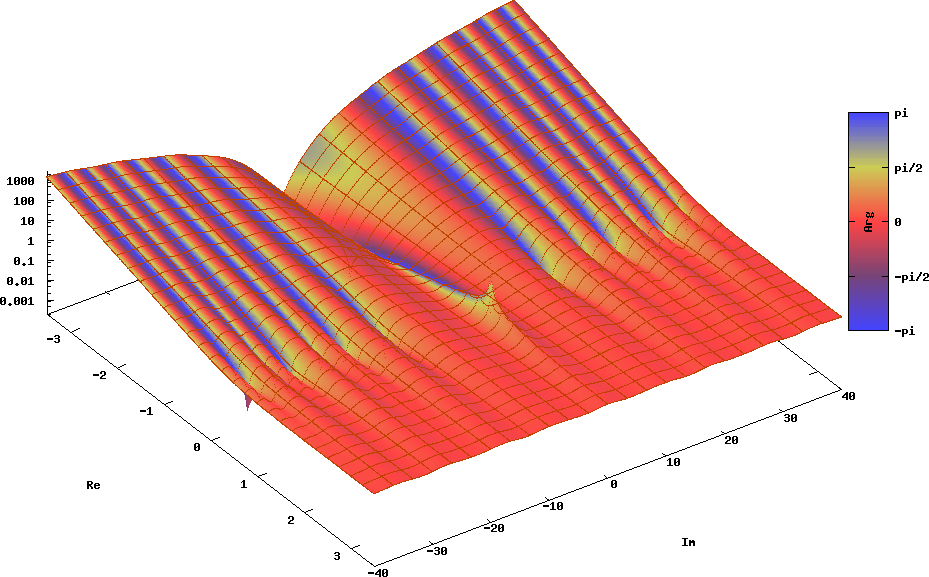
\includegraphics[width=60mm,height=36mm]{img/z/zwhole5.png}  
  \caption{     \label{fig:zeta}
    \emph{Funzione Zeta di Riemann} 
    $\zeta(s) = \sum_{n=1}^\infty \frac{1}{n^s}$, con $s = x+iy$ 
    nei domin\^{i} 
    $(x,y) \in [0,3]\times[-5,50]$ e
    $(x,y) \in \left[-\frac{7}{2}, \frac{7}{2}\right] \times \left[-40, 40\right]$
    (in quest'ultimo caso in scala logaritmica).
  }
\end{figure}
